\documentclass[12pt,a4paper]{report}
\usepackage[latin1]{inputenc}
\usepackage[spanish]{babel}
\usepackage{amsmath}
\usepackage{amsfonts}
\usepackage{amssymb}
\usepackage{graphicx}
\usepackage[left=2cm,right=2cm,top=2cm,bottom=2cm]{geometry}
\author{Oscar Cruz Cervantes}
\title{EV.2_2 Arreglos y Parametro s de los Amplificadores Clase A}


\begin{document}

\begin{center}
EV. 2.2\\
Arreglos y Parametro s de los Amplificadores Clase A\\
Oscar Cruz Cervantes\\
\end{center}
\begin{center}

\includegraphics[scale=2]{01.png}
\end{center}
\begin{center}
Sistemas electronicos de interfaz\\
Ing. Mecatronica 4ºB
\end{center}
\newpage
\section{Amplificadores Clase A}
los amplificadores clase A tienen la caracteristica de mantener una mayor fidelidad cuando el circuito esta polarizado, esto lo logras cuando logras que el voltaje entre el emizor y el colector es la mitad que el de la fuente.
Los amplificadores clase A a diferencia de los amplificadores normales resisten y requieren una mayor cantidad de corriente, esto es debido a que pueden aplifican las odas aun mas.
\begin{center}
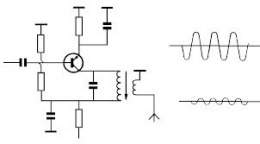
\includegraphics[scale=1.5]{02.jpg}
\end{center}
\subsection{Caracteristicas}
-Debido a que estos amplificadires son casi lineales tienen muy buena  fidelidad.\\
-Este amplificador tiende a presentar unas grandes y fuertes cantidades de calor. Sin embargo, los transistores de salida están siempre a una temperatura fija y sin alteraciones.\\
-La gran desventaja de los amplificadores clase A es que son poco eficientes, se requieren amplificadores muy grandes para dar 50W, y ese amplificador usa mucha corriente y se pone a muy alta temperatura.\\
\end{document}